
\section{Evaluation}
\label{sect:exper}

We have implemented a snapshot deduplication scheme on the Aliyun's cloud platform.
Our experimental evaluation has the following two objectives:
1) Analyze the commonality of content data blocks and the popularity  of hot items. We 
examine the impacts of CDS size on deduplication ratio.
2) Assess the effectiveness  of 3-level deduplication for reducing the storage requirement of snapshot 
backup. 

\subsection{Experimental setup}

An Aliyun our target is to backup cluster with 1000 nodes
with 25 VMs on each.
We are running our deduplication/backup  service on 100 nodes.
Memory usage is about 150MB space per node during backup and
the CPU usage is very small during the experiments. 
Based on the data studied,  each VM has about  40GB of storage  data usage on average,
OS disk and data disk each takes about 50\% of storage space.
The backup of VM snapshots is completed within two hours  every day,
and that translates to a backup throughput of 139GB per second, or 500TB per hour.
For each VM, the system keeps 10 automatically-backed snapshots in the storage while
a user may instruct extra snapshots to be saved.

% the system must finish saving daily snapshots of all VMs in 2 hours. In our typical 1000 nodes cluster, each node hosts 25 VMs, each VM has 40GB of data on average, that translates to backup throughput of 139GB/second, or 500TB/hour.

%In our snapshot deduplication architecture, CDS is the key to achieve greater deduplication than
%incremental backup solutions. Our basic assumption of CDS us that VM disks, especially OS disks,
%have huge amount of data in common, and such common data can be represented by a relatively smaller data set
%because of their high appearence frequency. As a result, the major portion of snapshot deduplication effect shall 
%emerge from eliminating the duplication of such a small data set. In this section, we evaluate
%the effectiveness of CDS using real user VM disks from our production VM cluster.

We have used a storage dataset of  1323 VM users collected from 100 Aliyun's cloud nodes to evaluate the effectiveness.
In this dataset, there are 10 snapshots per each VM user and the total amount of space investigated 
is 23.5 terabytes.
Each VM file is  divided into content blocks of
variable sizes~\cite{similar94,rabin81} with an average size of 4KB. 
The signature for variable-sized blocks is computed using  their SHA-1 hash. 
Each segment is of size 2MB.  
Popularity is computed by using 90\% of dataset, which reflects our setting that the system recomputes
CDS every 1-2 days to catch up the popularity trend.

%seg, and we performed global perfect deduplication 
%to caculate the number of duplicate copies of each individual unique block. We choose 2KB, 4KB, 16KB as the minimum, average
%and maximum block size
%OS data
%user data: zipf
%prediction
%say something about aliyun


%To compare the effectiveness with a full deduplication approach with an approximation,
%we use  extreme binning and perfect deduplication~\cite{extreme_binning09}. 
%For perfect deduplication and extreme binning, each snapshot is also divided into chunk blocks
%using TTTD with an average size of 4KB. The original extreme binning work uses the whole file
%as the input unit and  this size is too big in our system. 
%Thus we split each image snapshot file into variable-sized segments base on the block hash list, 
%using TTTD with average size of 2MB.

\subsection{Effectiveness of 3-level Deduplication}

\begin{figure}
  \centering
  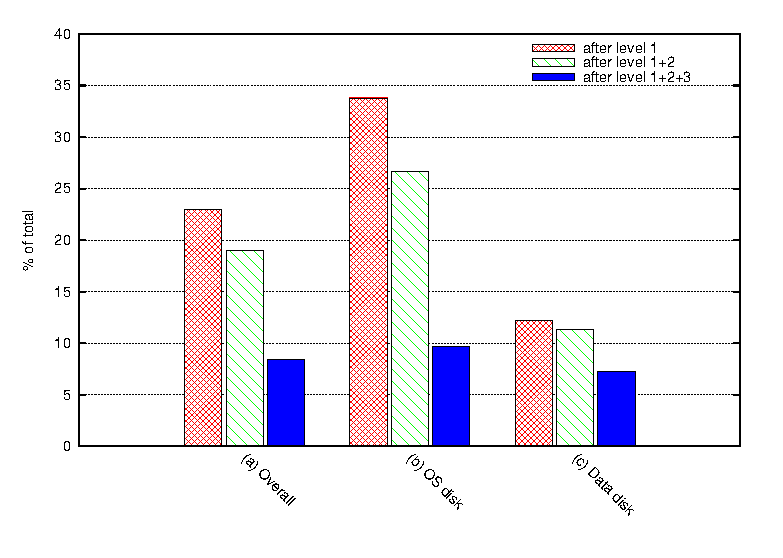
\epsfig{file=images/overall_effect.eps, width=3.5in}
  \caption{Impacts of 3-level deduplication. The height of each bar is the data size after 
deduplication divided by the original data size and the unit is percentage. }

  \label{fig:overall}
\end{figure}

Figure~\ref{fig:overall} shows the overall impact of 3-level deduplication.
The X axis shows the overall impact in (a),  impact on OS disk in (b), and impact on data disk in (c).
Each bar in the Y axis shows the data size after deduplication divided by the original data size.
Level-1 elimination can reduce the data size to about 22\% of original data, namely it delivers close 78\% reduction.
Level-2 elimination applied after level 1
reduces the size further to about 18.5\% of original size, namely it delivers additional 4.5\% reduction.
Level-3 elimination together with level 1 and 2
reduces the size further to 8\% of original size, namely it delivers additional 10.5\% reduction.
Level 2 elimination is more visible in OS disk than data disk, because data change frequency is really small
when we sample last 10 snapshots of each user in 10 days. Nevertheless, the overall impact of level 2 is still significant.
A 4.5\% of reduction from the original data represents about 450TB space saving for a 1000-node cluster.


\begin{figure}
  \centering
 %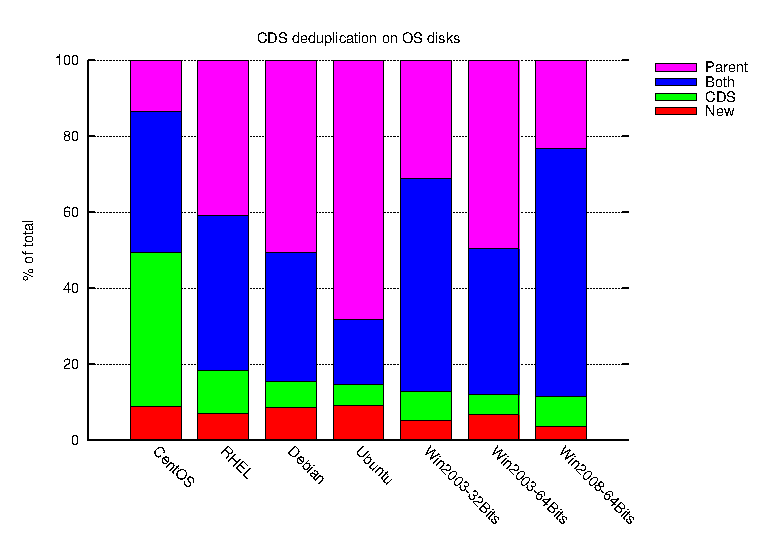
\epsfig{file=images/os_cds_sim.eps, width=3in}
  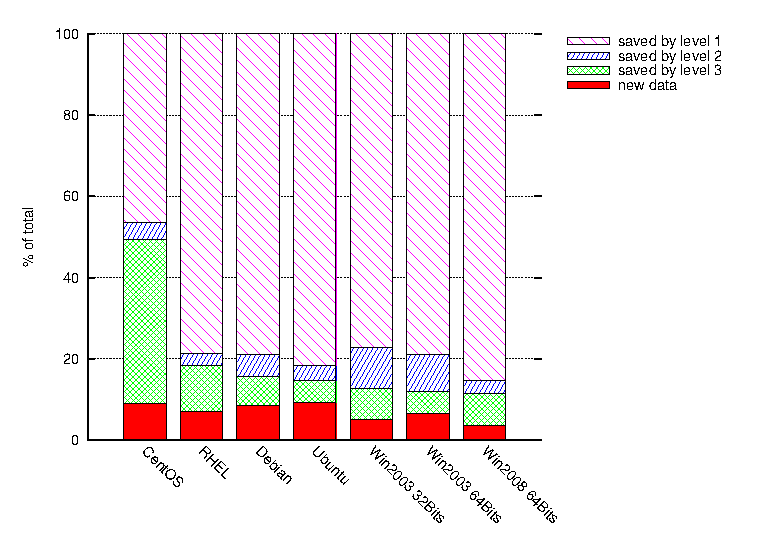
\epsfig{file=images/3level_os.eps, width=3.5in}
  \caption{Impact of 3-level deduplication for OS releases.}
  \label{fig:oscds}
\end{figure}

To see the impact of multi-level deduplication on different OS releases, we choose 7 major OSes in Aliyun's
VM cloud platform and they are: 
Win2008 Server 64 bits, Win2003 Server 32 bits, Win2003 Server 64 bits, RHEL, CentOS, Ubuntu Server and Debian (all Linux
distributions are 64 bits).
Then we examine 5 VM user disks from each OS, and 10 snapshots for each VM. These VMs have been actively used by their
owners. 
%Some of  OS disks are modified frequently and in some cases,  users even store a large amount of user data on
Figure~\ref{fig:oscds} shows the impact of different levels of deduplication for different OS releases.
In this experiment, we tag each block as  ``new''
if this block cannot be deduplicated by our scheme and thus has to be written to the snapshot block store;
``CDS''  if this block can be found  in CDS;
``Parent segment'' if  this block is marked unchanged in parent's segment recipe.
``Parent block'' if  this block is marked unchanged in parent's block recipe.
With this tagging, we compute the percentage of duplication accomplished by level-1 inner VM deduplication,
level-2 inner VM deduplication and level 3 cross-VM deduplication.
As we can see from Figure~\ref{fig:oscds}, level-1 deduplication accomplishes a large percentage of elimination
this is because the time interval between two snapshots in our dataset
is quite short and the Aliyun cloud service makes a snapshot  everyday  for each VM.
On the other hand,  CDS still finds lots of duplicates that inner VM deduplication can't find,
contributing about about 10\% of reduction on average.

%Combining OS disks in all the VMs, we see the overall 7.4TB of data is reduced to 512GB. 
%The extreme binning approach can reduce this data set to 542GB, which is slightly worse. As a reference, 
%perfect deduplication achieves 364GB in this experiment.

%Overall speaking, inner   VM deduplication or  CDS-based deduplication
%can work well alone, but by combining them together we get a fairly good and stable deduplication ratio to 
%all kind of OSes. 
%Compared to a traditional dirty bit approach based on pages of
%each file (e.g. segment in our scheme),
%our CDS-based level 3 approach  can save additional 50\% storage space because many of level 2 block
%content can be eliminated using the CDS also.

\subsection{Coverage of common data blocks}

%We study characteristics of common data blocks among snapshots of VM users
%and examine the impacts if we only store a relative small amount of common data blocks to be sored in the CDS server.
%There are two advantages to exploit this.
%First, a smaller CDS reduces overall resource requirement while covering  most of data blocks in snapshots.
%Second a smaller CDS makes the fault tolerance management  easier because we can replicate  more copies
%to mitigate the failure.

%We consider each virtual disk contains two parts: OS partition and regular user data partition
%and study their characteristics seperately.
%In Aliyun's VM cloud, each VM explicitly maintains  one OS disk, plus  one or more data disks.
%During VM's creation, its OS disk is directly copied from user's choosen base image.
%Since  they dare brought by the operating system and popular 
%software installations,  they are rarely modified or deleted.
%base image data as a hint.
%Through users may change configurations, install software, or write user data into OS disk,
%but most of the OS related data shall keep unchanged. 

%Previous study has also supported this\cite{vmimage}. Therefore, we can let all OS disks share these
%common data in their snapshot backups.
%We choose user's data disks rather than OS disks in thie experiment for several reasons: First, the data in OS disks are 
%instinctively highly similar, because most of the VM users only make some common or unique but tiny changes to their OSes,
%so the data duplication pattern in OS disks cannot reflect the real distribution of general user data.
%Second, the data disks are way more important in terms of data safty and backup because they are 
%what users really care about.

%Furthermore, our study on user's data disks has shown that the duplication pattern of
%variable-sized data blocks follows \emph{Zipf-like} distribution. As a result, the major portion of 
%deduplication effect will emerge from eliminating the duplication of frequently seen data.
%define CDS


\comments{
\begin{figure}[htbp]
\centering
%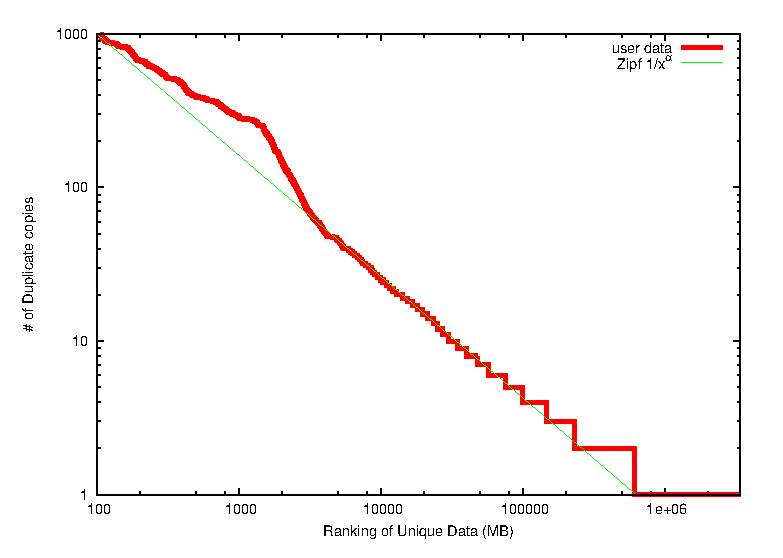
\epsfig{file=images/log-log.disk.eps, height=2in, width=2.66in}
%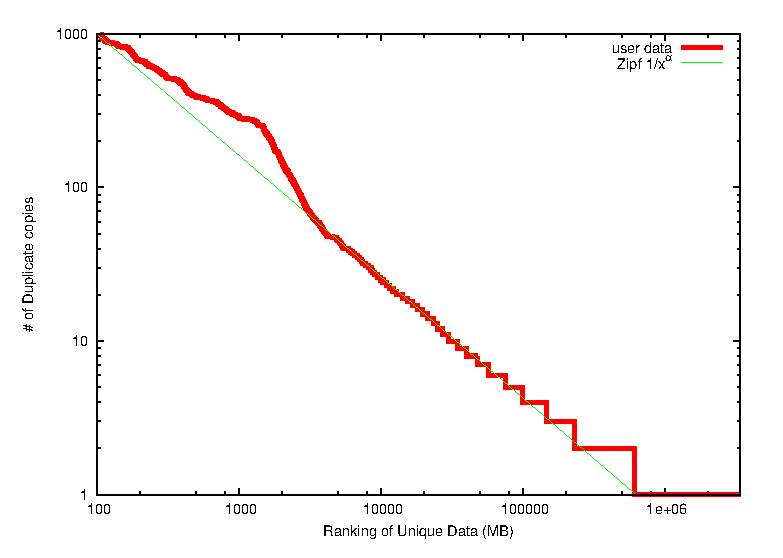
\epsfig{file=images/log-log.disk.eps, width=3in}
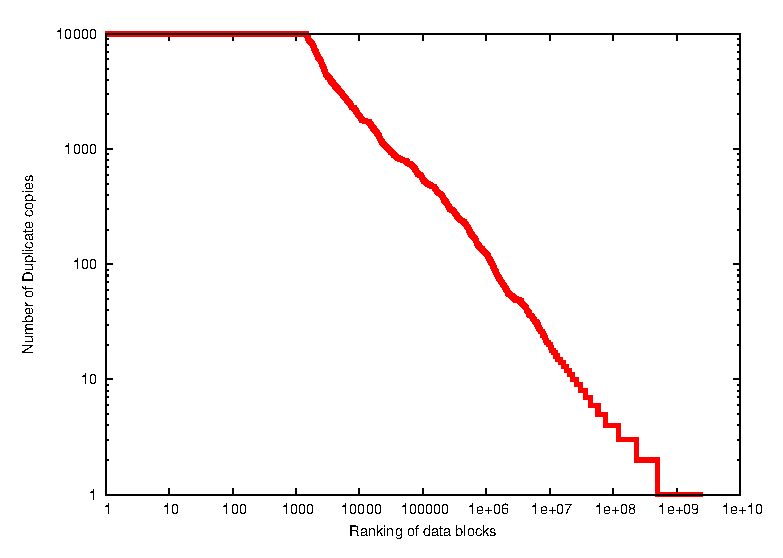
\epsfig{file=images/datadisk.count_rank.eps, width=3.5in}
\caption{Duplicate count  of common data blocks in a log scale.}
\label{fig:zipf-data}
\end{figure}
Figure \ref{fig:zipf-data} shows the duplicate count  for different data blocks sorted by their ranking in 
terms of the duplication count. $Y$ axis is the popularity of a data block in a log scale 
measured its duplicate count among snapshots. $X$ axis is the identification of data blocks in a log scale
sorted by their duplicate rank.  The rank number  1  is the block with the highest number of duplicates.
The curve exhibits that the popularity of common data blocks partially follows a  Zipf-like distribution.

\begin{figure}
\centering
%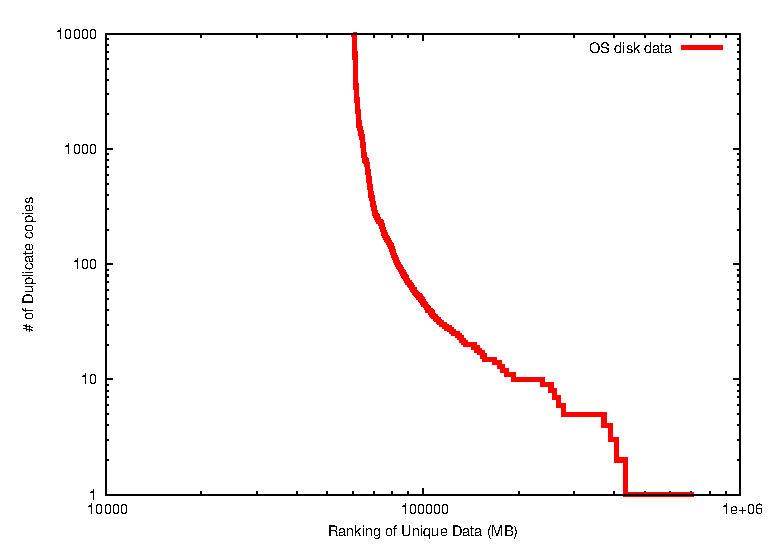
\epsfig{file=images/log-log.35vmos.eps,  width=3in}
%\epsfig{file=images/35os.count_rank.eps, width=3in}
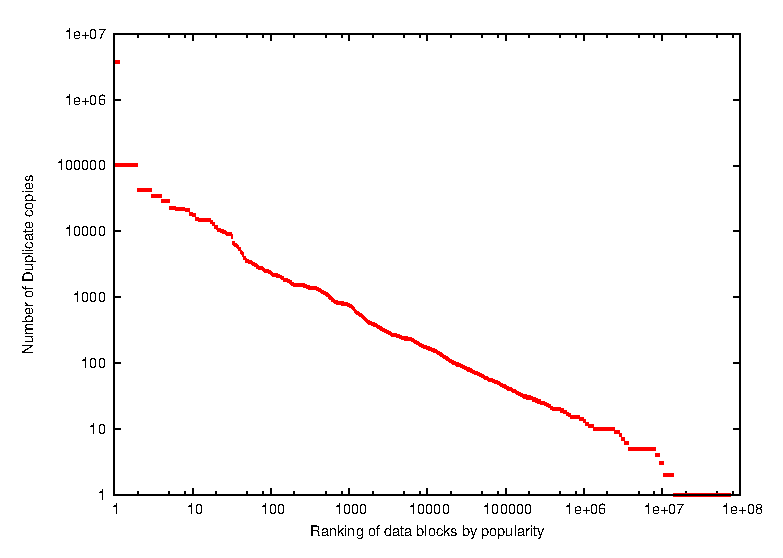
\epsfig{file=images/35vmos.count-rank.eps,width=3.5in}
\caption{ Duplicate count of  common OS blocks in a log scale.}
\label{fig:OSpopular}
\end{figure}
Figure \ref{fig:OSpopular} shows the duplicate count  for OS disk snapshot blocks sorted by their ranking.
$Y$ axis is the popularity of an OS block in a log scale 
measured its duplicate count among snapshots. $X$ axis is the identification of OS blocks in a log scale
sorted by their duplicate rank.  For the top ranked blocks, there is a flat line in terms of duplicate counts. That
is because there are a large number of OS blocks which have appear in all copies of such OS releases.

}

 
\begin{figure}
\centering
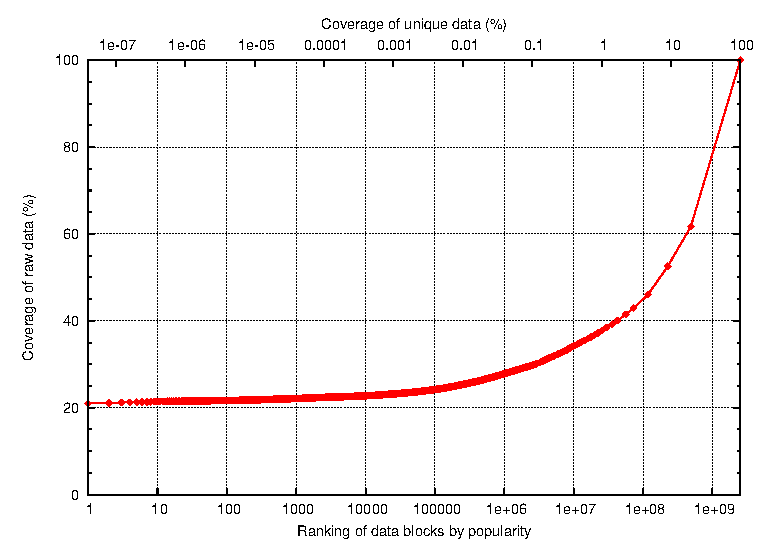
\epsfig{file=images/ay41a_big.data_disk.cdf.eps, width=3.5in}
%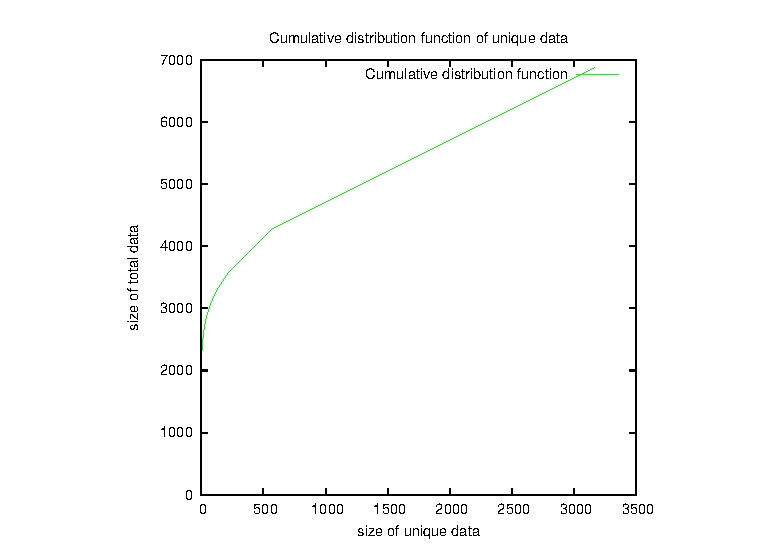
\epsfig{file=images/cdf.disk.v4.eps, width=3in}
%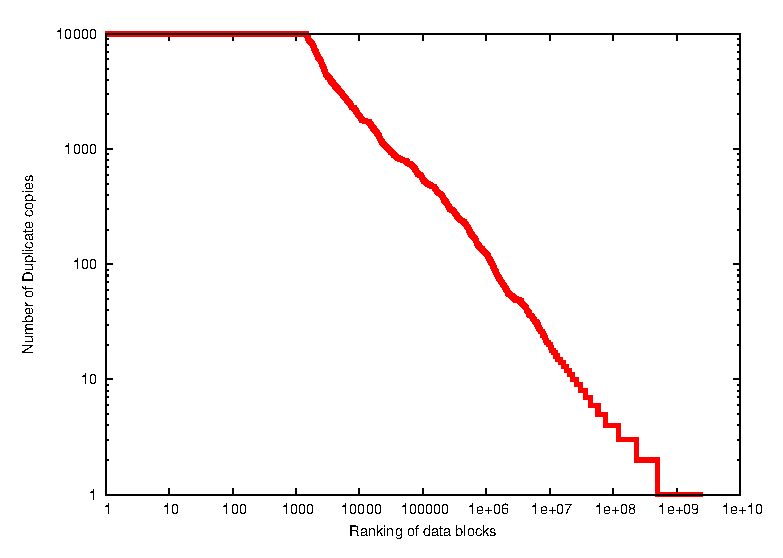
\epsfig{file=images/datadisk.count_rank.eps, width=3in}
%\epsfig{file=images/35os.count_rank.eps, width=3in}

\caption{Cumulative  coverage of popular common user data blocks.}
\label{fig:userdatacoverage}
\end{figure}

We further study how CDS covers content blocks used in image files using 90\% of
the collected dataset.
Figure \ref{fig:userdatacoverage} shows the cumulative coverage  ratio of  popular common user data blocks. 
The $X$ axis is the rank of common user data blocks.
Let $S_i$ and $F_I$ be the size and duplicate count 
of the $i$-th block ranked by its duplicate rank.  Then $Y$ axis is the coverage of
the common dataset covering data items from rank 1 to rank $i$. Namely  
\[
\frac{ \sum_{i=1}^{i} S_i * F_i} {\mbox{Total data size}}.
\]

Thus with about 1\% of blocks on data disks, CDS can cover about 38\% of total data blocks
appeared in in all data snapshots. The corresponding CDS index uses about 150MB memory per machine.

%Figure~\ref{fig:OSdatacoverage} shows the cumulative coverage  ratio of  popular common OS blocks. 
%From both graphs, a small number of most popular common blocks can coverage a large percentage of 
%snapshot blocks and thus the size of CDS can be chosen to be small while still having a large
%coverage. 

%\begin{figure}
%\centering
%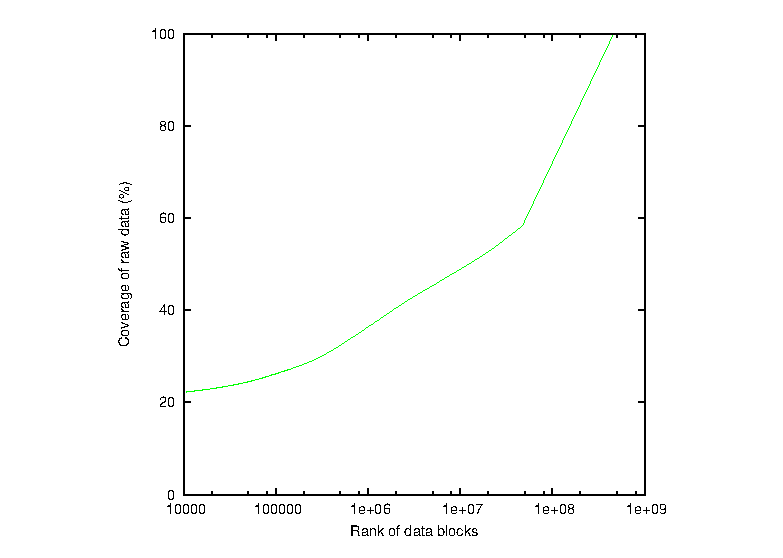
\epsfig{file=images/ay41a_small.os_incremental.cdf.eps, width=3in}
%\caption{ Cumulative  coverage of popular common OS disk blocks.}
%\label{fig:OSdatacoverage}
%\end{figure}


%We define \emph{OS CDS} to be the unchanged data across the base VM image and the snapshots of all
%OS disks which are derived from it. Such data are brought by the operating system and popular 
%software installations, they are rarely modified or deleted, and can be easily extracted using 
%base image data as a hint.


Because there are a limited number of OS releases supported by Aliyun, we study common blocks  among
OS disks loaded with  the same OS release. 
%The selection of CDS is completed by separating OS disk and data disk.
%While block commonality among data disks may be affected in some degree
% when we scale up the number of total VMs  to be supported,
%we expect that  the block commonality among OS disks still remains to be high and  
%%can be well covered by a fixed CDS because users still adopt common OS releases.
%we choose 7 major OSes in Aliyun's
%VM cloud platform and they are: 
%Win2008 Server 64 bits, Win2003 Server 32 bits, Win2003 Server 64 bits, RHEL, CentOS, Ubuntu Server and Debian (all Linux
%distributions are 64 bits).
%we examine 5 VM user disks from each OS, and 10 snapshots for each VM. These VMs have been actively used by their
%owners. Some of  OS disks are modified frequently and in some cases,  users even store a large amount of user data on
%their OS disks. 
%For example, some Ubuntu OS disks have only 2GB of data while some have 50GB.
%For each OS, the base image and all OS
%disk snapshots are divided into variable-sized blocks. Then 
In  Figure~\ref{fig:OSunchanged},  we list a conservative  commonality study in 7 major OS versions  supported
in Aliyun.  We consider the earlier snapshot for each OS disk as the base image.
For every block in the base image, we classify this block as ``completely common''
if  this block has appeared in all snapshots of the same OS release even they are used by different VMs.
Figure \ref{fig:OSunchanged} shows that for each
OS,  at least 70\% of OS blocks are completely common among all snapshots of the same OS. 
Some latest release  of OS tends to have a higher percentage of content change
while  old release tends to have more variations of content versions.
That can be interpreted as that users with very old  version of operating systems
have a lower tendency to update their OS versions and this causes a larger discrepancy
among OS snapshots of these users.

%into the unchanged category of OS data.

\begin{figure}
\centering
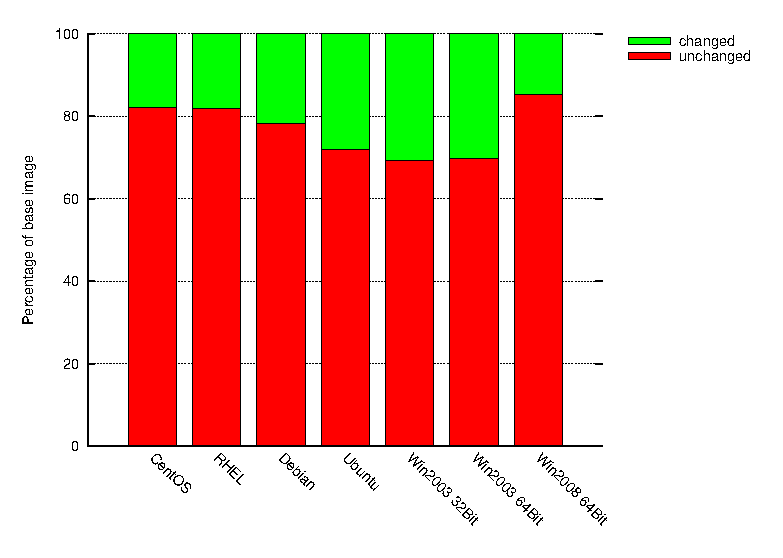
\epsfig{file=images/os_subset.eps, width=3.5in}
\caption{Percentage of completely common blocks among different VMs for the same OS release.}
\label{fig:OSunchanged}
\end{figure}

Based on the above analysis, we have selected a small set of most popular
OS blocks, which is about 100GB OS data and its corresponding CDS index takes about 1GB memory space in total.
They can cover sufficiently over 70\% of OS blocks.

%Then we use this CDS to run the deduplication process again.
%That correspond to about  80GB of OS blocks and its corresponding CDS meta occupies 800MB in the cache.
%  data from 350 OS disk snapshots,

%The above analysis is only an estimation of OS and software related common data, 
%some user installed software may not be discovered by this method because they are not 
%included in the base image. However, as we can see in the next section, 
%the overall duplication of user generated data
%follows the Zipf-like distribution, thus all popular data can be discovered by statistic analysis.


%Zipf's law has been shown to characterize use of words in a natural language, city populations, 
%popularity of website visits and other internet traffic data.

%Here we present the first fully consistent empirical study showing that data duplication
%pattern in very large scale storage follows Zipf-like distribution. More specifically,
%we show that the duplication count of any unique data block is inversely proportional to its rank
%in the frequency table, with $\alpha$ smaller than unity. 
%As far as we know, this is the first study of large scale real user data to disclose
%the Zipf-like distribution pattern in data storage area.

%\subsubsection{The model}
%Consider a general storage system that holds user's files without any deduplication. 
%Let $N$ be the total number of unique data blocks after 
%content-defined chunking and deduplication, 
%$C_N(i)$ be the number of duplicate copies that the $i$th data block being
%stored in storage, given all the unique data blocks be ranked in order of their number of duplicate copies.
%Let $S_i$ be the size of $i$th block,
%then the actual ranking of the $i$th block is reflected by $\sum_{1}^{i-1}S_i$. 

%\subsubsection{Methodology}
%1323 users' virtual data disks were scanned using TTTD content-defined chunking, and we performed global perfect deduplication 
%to caculate the number of duplicate copies of each individual unique block. We choose 2KB, 4KB, 16KB as the minimum, average
%and maximum block size, all variable-sized blocks are compared by their SHA-1 hash arther than real data.
%
%We choose user's data disks rather than OS disks in thie experiment for several reasons: First, the data in OS disks are 
%instinctively highly similar, because most of the VM users only make some common or unique but tiny changes to their OSes,
%so the data duplication pattern in OS disks cannot reflect the real distribution of general user data.
%Second, the data disks are way more important in terms of data safty and backup because they are 
%what users really care about.

\comments{
\subsection{Discussion}
By storing the hash index of a small set of hottest data (CDS), we expect to achieve great 
deduplication effect with minimal cost.
But one problem of the CDS is what we called \emph{blind spot}: the update of CDS is always 
behind new data's arrival,
as a result, some data must have been written to the backup store before being collected into CDS, thus such 
duplication may comprise the effect of
CDS. For instance, when a MySQL update is released, some users may apply it very quickly, so the new hot data bring by
this update will not be filtered by CDS. Only until later our CDS update includes those new data, then the rest of MySQL users get benefited.
We can take a few measurements to reduce the impact of blind spot. First, the data in blind spot will not accumulate, because snapshots backup
is a paid service, so over the long term, data in blind spot will be removed from backup store as VMs and old snapshots keep being deleted.
Second, for the major OS updates, we can anticipate them in advance by putting the new hot data into CDS before users widely adopt them.

Another problem associated with CDS is that some data in CDS may no longer be popular or even disappear
as time goes. For example, an MySQL software update may invalidate some data that we previously hold in 
the CDS. If some data blocks in CDS are no longer referenced, our map-reduce process is able to detect
this situation, so invalid data will be removed and new data will be added during the next CDS update. 
But if some users choose to keep their old MySQL version, then the corresponding old and new data will co-exist in the CDS.
}



%In our snapshot deduplication architecture, CDS is the key to achieve greater deduplication than
%incremental backup solutions. Our basic assumption of CDS us that VM disks, especially OS disks,
%have huge amount of data in common, and such common data can be represented by a relatively smaller data set
%because of their high appearence frequency. As a result, the major portion of snapshot deduplication effect shall 
%emerge from eliminating the duplication of such a small data set. In this section, we evaluate
%the effectiveness of CDS using real user VM disks from our production VM cluster.


\subsection{A comparison of perfect and CDS-based deduplication }
%Figure~\ref{fig:pd} shows the compression ratio of perfect deduplication at different dataset sizes
%as we vary the data size from about 4 terabytes to about 23.5 terabytes.
After level-1 and level 2 elimination, our experiment shows that 
the full deduplication would reduce the storage  further   by  45\% to 53\% of user disk space. 
If we put all these unique data into CDS, we could achieve full deduplication,
but the CDS size is not affordable. So we evaluate how much space saving of 
deduplication can be achieved when varying the CDS size.
%\begin{figure}
%  \centering
%  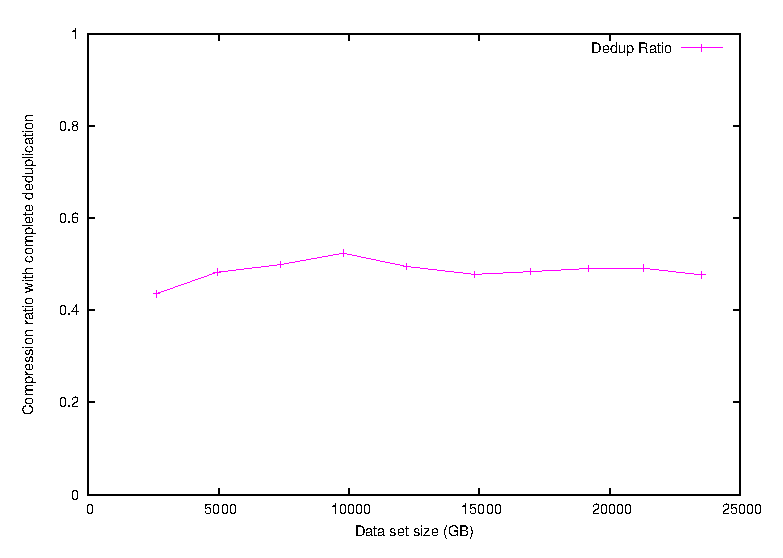
\epsfig{file=images/dedup_ratio.eps, height=2in, width=2.66in}
%  \caption{Perfect deduplication on data disks}
%  \label{fig:pd}
%\end{figure}

%We rank unique data blocks by their duplication count, and choose the hottest blocks as CDS. 
Figure \ref{fig:datacdssize} shows the relationship between CDS cache size and relative space saving ratio
compared to the full deduplication.  The unit of CDS size is gigabytes.
We define \emph{space saving ratio} as the space saving of the CDS method divided by 
full deduplication saving ratio. 
With a 100GB CDS data (namely 1GB CDS index) can still  accomplish about 75\% 
of what perfect deduplication can do.
%But this effect decreases when more data are added to CDS. 
%The lower bound of CDS space saving ratio is 50\%, which is very easy to accomplish. 

\begin{figure}
  \centering
  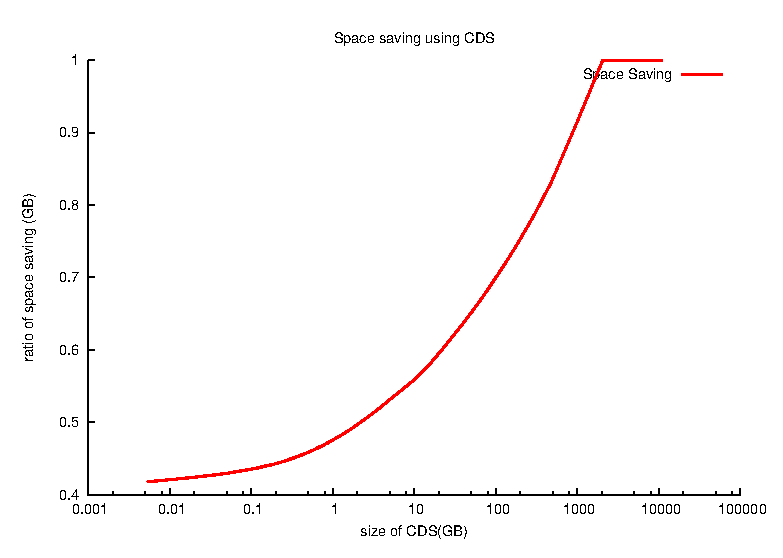
\epsfig{file=images/uniquedata-saving.eps, width=3.5in}
  \caption{Relative ratio of space size compared to full deduplication when CDS size changes.}
  \label{fig:datacdssize}
\end{figure}

%CDS size is restricted by system memory resource.
Figure \ref{fig:datacds} shows how CDS space saving ratio
compared to the full deduplication is affected by the dataset size. 
The calculation is done after level 1 and level 2 deduplication.
$X$ axis uses the data size collected  from up to 1323 VMs, which occupies about
53 machines. 
In this experiment we first set out a goal of space saving ratio completed, 
then watch how much data needs to be placed in CDS cache to achieve this goal.
From the graph we can see a 75\% saving ratio lead to a stable ratio between 
CDS size and data size, which requires 1\% of data to be placed in CDS.

When we deal with a cluster of 1,000 nodes, we expect that using
1\% of data disks can cover more what we have seen from this
1323 VM dataset, assuming that the average behavior of every subcluster with 53 machines
exhibits a similar commonality. 
In addition to this, CDS for OS disks will become even more effective when
there are more VMs sharing the same collection of OS releases. 
%Base on above data we can estimate the size of data CDS and its effect. 
%Currently we prepared 500MB memory per machine to store CDS meta, then it can represent 50GB of data. 
%If we assume each VM has 30GB of user data at runtime, and we host 25 VMs per machine, 
% maintain 10 snapshots per VM, each brings 10\% additional modified data. 
%Thus the user data in snapshot system is 1.5TB per machine. So the upper bound of 
%$CDS size/ Data size = 0.033$, which is sufficient for the 75\% saving goal.

\begin{figure}
  \centering
  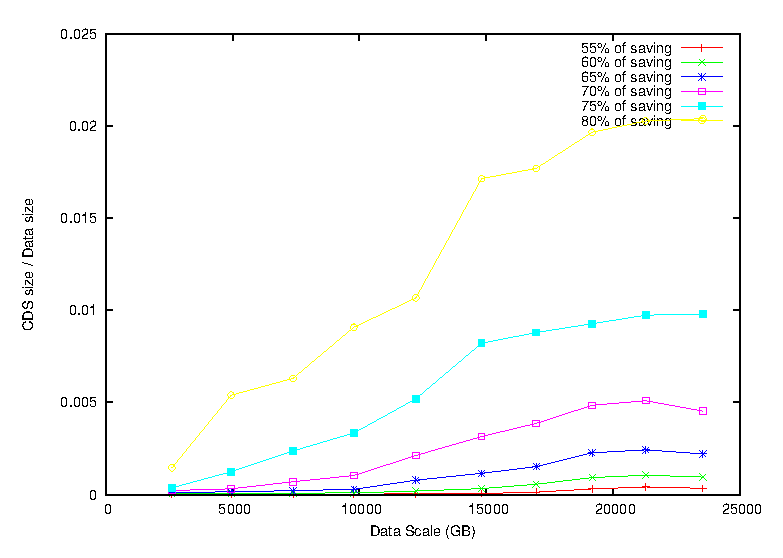
\epsfig{file=images/cds_scale.0.7.eps, width=3.5in}
  \caption{The relative size ratio of  CDS over the data size. }
  \label{fig:datacds}
\end{figure}

%Unlike the CDS of OS disks which is mainly composed of OS related data thus highly predictable, 
%data disks is unpredictable because we cannot control what user can put in there. But we still
%suspect that highly duplicated data in existing data are very likely to be duplicated again.
%So we randomly pick 50 out of 1322 data disks as the new data, and use the rest as existing data
%to extract CDS. Using 1.5\% as CDS threshold, we see the total 1198GB of new data is reduced by 
%755.8GB, while perfect deduplication can reduce 1017.4GB. So 74.3\% of duplicate blocks are eliminated 
%by pre-trained CDS, which is quite satisfactory.
